\documentclass[12pt, a4paper]{article}
\usepackage{amssymb}
\usepackage{url}
\usepackage[colorlinks=false]{hyperref}
\PassOptionsToPackage{hyphens}{url}
\usepackage[utf8]{inputenc}
\usepackage{enumitem}
\usepackage{indentfirst}
\usepackage{listings}
\usepackage{graphicx}
\usepackage{color}
\usepackage{xcolor}
\usepackage{listings}
\usepackage{xparse}
\usepackage{subcaption}
\usepackage{cleveref}

\captionsetup[subfigure]{subrefformat=simple,labelformat=simple}
\renewcommand\thesubfigure{(\alph{subfigure})}

\usepackage[portuguese]{babel}
\usepackage{geometry}
\geometry{legalpaper, a4paper,
 total={170mm,257mm},
 left=20mm,
 top=20mm}
\setlength{\voffset}{-10mm}
\definecolor{dkgreen}{rgb}{0,0.6,0}
\definecolor{gray}{rgb}{0.5,0.5,0.5}
\definecolor{mauve}{rgb}{0.58,0,0.82}

\lstdefinestyle{Java}{frame=tb,
  language=Java,
  aboveskip=3mm,
  belowskip=3mm,
  showstringspaces=false,
  columns=flexible,
  basicstyle={\small\ttfamily},
  numbers=none,
  numberstyle=\tiny\color{gray},
  keywordstyle=\color{blue},
  commentstyle=\color{dkgreen},
  stringstyle=\color{mauve},
  breaklines=true,
  breakatwhitespace=true,
  tabsize=3
}


\lstdefinestyle{Xml}{frame=tb,
  language=Xml,
  aboveskip=3mm,
  belowskip=3mm,
  showstringspaces=false,
  columns=flexible,
  basicstyle={\small\ttfamily},
  numbers=none,
  numberstyle=\tiny\color{gray},
  keywordstyle=\color{blue},
  commentstyle=\color{dkgreen},
  stringstyle=\color{mauve},
  breaklines=true,
  breakatwhitespace=true,
  tabsize=3
}

\usepackage[num,overcite]{abntex2cite}
\citebrackets[]

\NewDocumentCommand{\codeword}{v}{
    \texttt{\textcolor{blue}{#1}}
}

\newcommand{\TitleAndSubtitle}[2]{\title{#1 \\ \large{#2}}}

\newcommand{\tit}[1]{\textit{#1}}
\newcommand{\tb}[1]{\textbf{#1}}
\newcommand{\tbi}[1]{\textbf{\textit{#1}}}

\newcommand{\bitem}[1]{\tb{(\tit{#1})}}
\newcommand{\iitem}[1]{(\tit{#1})}

\newcommand{\sw}{\tit{software}}
\newcommand{\kernel}{\tit{kernel}}
\newcommand{\Kernel}{\tit{Kernel}}
\newcommand{\mobile}{\tit{mobile}}

\newcommand{\quotes}[1]{``#1''}

\TitleAndSubtitle{Sistemas Operacionais I N}{Estudo de Caso: Políticas de Processos no Android}
\author{Wellington Espindula}
\date{Setembro de 2021}

\begin{document}
    \maketitle
   
   \section{Implementação de Processos e Escalonador}
   O Sistema Operacional Android - mantido pela Open Handset Alliance e pela Google LLC - é o sistema operacional \mobile \ mais utilizado em todo o mundo, sendo executado nos mais diversos tipos de dispositivos, tais como Smartphones, Tables, Smartwatches e Smart TV's.\cite{wiki:android} Para tanto, este é composto de um \kernel \ desenvolvido pelo próprio Android, conhecido como Android Commom Kernel (ou ACK), que é, de forma simples, o \kernel \ comum para todos os dispositivos. Este posteriormente pode ser modificado pelos fornecedores e para o dispositivo, ativando periféricos e \tit{drivers} adicionais e personalizações. O ACK, por sua vez, é um \tit{fork} do \kernel \ Linux LTS. Na sua versão mais nova, Android 12, a \tit{release} utiliza o \kernel \ Linux 5.2 e 5.10.\cite{android:generic-kernel-image} Na figura \ref{fig:android-kernel-development}, pode-se visualizar a hierarquia de desenvolvimento do \kernel.
    \begin{figure}[!ht]
        \centering
        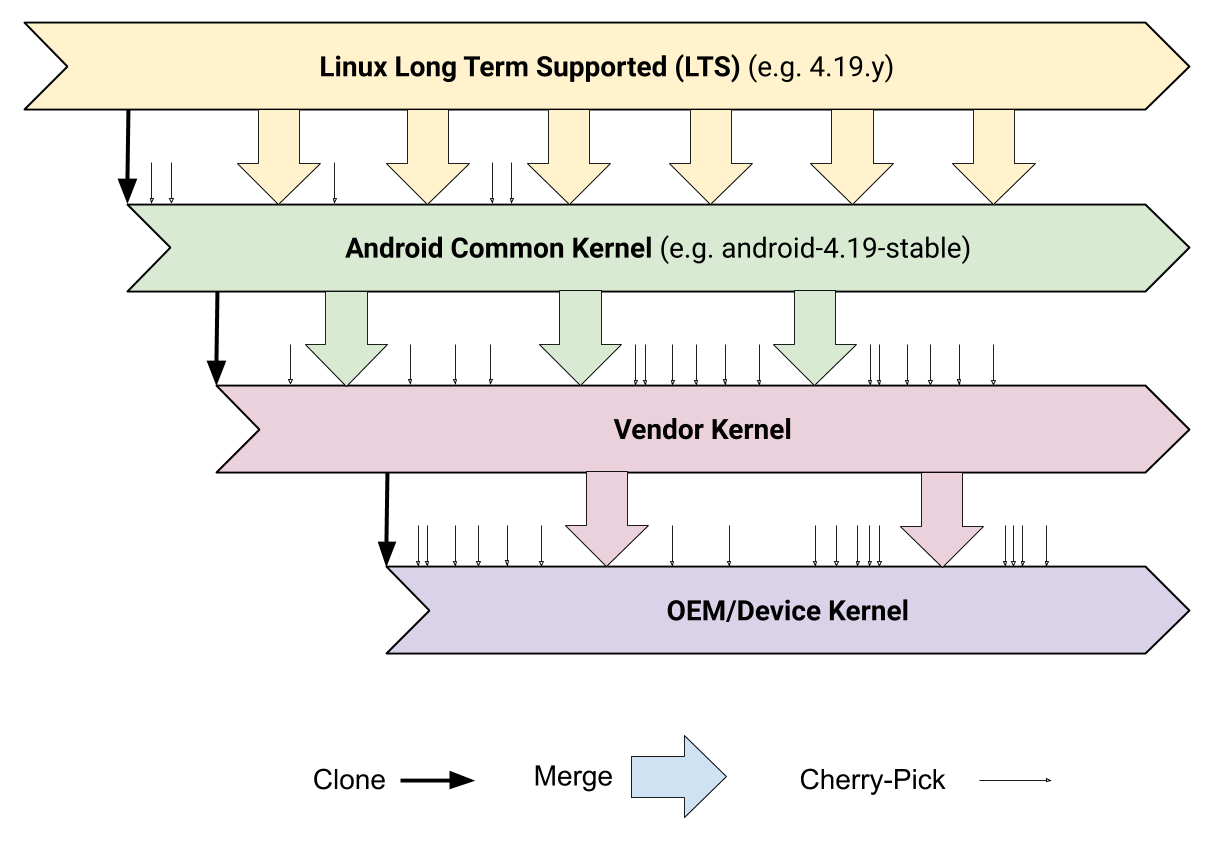
\includegraphics[width=\textwidth,height=0.30\textheight,keepaspectratio]{generic-kernel-image-overview.png}
        \caption{Hierarquia do desenvolvimento do \Kernel \ Android. Fonte: Android Source (2021). Disponível em: \url{https://source.android.com/devices/architecture/kernel/generic-kernel-image}.}
        \label{fig:android-kernel-development}
    \end{figure}
    
    Por definição, um processo é uma instância de um programa em execução; deste modo, um papel principal dos sistemas operacionais é fornecer o suporte - através de rotinas - para criação, execução e gerenciamento os processo. Do ponto de vista de um sistema operacional, um processo pode ser representado através de uma estrutura de dados formado por, entre outros atributos, seu PID (identificador de processo), uma árvore Heap - que irá ser responsável por alocação de memória dinâmica -, uma pilha - que armazenará, por exemplo, variáveis locais e endereços de retorno de sub-rotinas - e informações de estado - Estado Atual, \tit{Program Counter}, Dados de Registradores.\cite{ArahamSilberschat2} Dito isso, existem diferentes algoritmos que implementam políticas de escalonamento do processos. O Android, por ter um \kernel \ derivado do Linux, apresenta o mesmo escalonador que este, de tal modo que o escalonador do Linux é incluído no \kernel \ do Android.\cite{android:sched_h}
    
    O \Kernel \ Linux, embora implemente diferentes políticas de escalonamento (como o \tit{Round-Robin} com \tit{Aging}), introduziu em sua versão 2.6.23 (2007) o algoritmo de escalonamento \tit{Completely Fair Schedule} (CFS) e internamente o CFS é o escalonador padrão, definido no cabeçalho com a macro \codeword{SCHED_NORMAL}.\cite{columbia:linux-sched, wiki:linux-kernel} O \tit{Round-Robin} e o CFS são ambos algoritmos de escalonamento preemptivos, o que significa que um processo pode ser interrompido para dar lugar à outro com a finalidade de maximizar a vazão de processos executados e o uso de CPU. O CFS modela um sistema multi-tarefas ideal e traz como benefícios a equidade de processos e a melhora da fluidez do sistema. Como contrapartida, o CFS tem complexidade $O(n)$ para encontrar o próximo processo.\cite{columbia:linux-sched}
    
    \section{Processos Android e Ciclo de Vida}
    A partir do Android 5.0, cada aplicativo Android é executado em um próprio processo Linux através de uma instância do \tit{Android Runtime} (ART). O processo é criado assim que alguma parte de seu código precisa ser executado e será mantido em execução até que este não seja mais necessário e o sistema reivindique a sua memória para executar outras aplicações.\cite{android:platform}
    
    Uma aplicação Android pode utilizar três tipos de componentes de aplicação. São esses \bitem{i} \tb{Activity} - Componente de Aplicação responsável por prover uma interface na qual usuários podem interagir com; \bitem{ii} \tb{Service} - Componente responsável por execução de operações de longa duração em plano de fundo, muito embora existam \tit{Foreground Services} que executam serviços em plano de fundo de forma notificável ao usuário; e \bitem{iii} \tb{BroadcastReceiver} - Receptor de eventos de sistema, tais como o \codeword{BOOT_COMPLETED}, \codeword{CALL} e \codeword{BATTERY_LOW}.
    
    A fim de determinar um nível de hierarquia de prioridade entre os processos, o Android determina os seguintes tipos de processos:\cite{android:proccess-lifecycle}
    \begin{enumerate}[label=\textbf{\arabic*.}]
        \item \tb{Processo em Primeiro Plano:} também conhecido como \tit{Foreground}, é aquele processo que é necessário para as atividades correntes do usuário e pode ser uma \tit{Activity} executando na parte visível da interface gráfica, um \tit{BroadcastReceiver} que está rodando o código de recebimento de evento e um \tit{Service} executando seu código de inicialização/destruição.
        \item \tb{Processo Visível:} realiza tarefas que mesmo não estejam em primeiro plano ou em execução direta, mas que o usuário está consciente de sua execução, como, por exemplo, quando uma \tit{Activity} foi pausada, quando existe uma \tit{Foreground Service} em execução ou quando algum serviço específico de sistema (desde que o usuário esteja ciente) está executando tal como um papel de parede \tit{live}.
        \item \tb{Serviço:} processos cuja execução não é visível para o usuário, muito embora sua execução seja importante para as aplicações. Alguns exemplos são serviços de sincronização e compressão de dados.
        \item \tb{Processo em Cache:} processo que não é mais necessário, mas que fica em \tit{cache} para execução mais rápida.
    \end{enumerate}
    
    Um ponto diferencial quando se fala em um sistema operacional \tit{mobile} em relação aos sistemas operacionais \tit{desktops} é que os recursos são bem mais escassos e este também acaba sendo responsável por gerenciar os recursos de forma a otimizá-los para os diferentes contextos dos usuários. Temos como exemplo de recursos a memória e a bateria de um \tit{smartphone} que o SO precisa gerenciar com muita cautela, habilitando e desabilitando serviços em diferentes cenários, a fim de maximizar a experiência do usuário.
    
    Por conseguinte, esta hierarquia faz-se importante não apenas a nível de escalonamento de processos, mas também em termos de distribuição de recursos. Portanto, ela também é utilizada quando é necessário determinar qual processo precisa ser matado em condições de baixa memória disponível.\cite{android:proccess-lifecycle}
   
    
    % Doze mode
    
    % Services that have been running for a long time (such as 30 minutes or more) may be demoted in importance to allow their process to drop to the cached list described next. This helps avoid situations where long running services that use excessive resources (for example, by leaking memory) prevent the system from delivering a good user experience.
        
    
    \subsection{Do ponto de vista do Desenvolvedor de Sistemas}
    Assim como supracitado ao longo do texto, cada aplicação Android roda seu próprio processo. Então o desenvolvimento de sistemas em Android perpassa sempre o Android SDK; este, através de suas APIs, dará a interface para a criação e gerenciamento de processos dentro de um ponto de vista de um desenvolvedor. Vale relembrar e ressaltar também que as aplicações executam dentro do ART. Através dessa perspectiva, nota-se que o desenvolvedor não mais poderá realizar chamadas de criação de processos e comunicação intra-processual de forma nativa, mas, sim, precisará de um respaldo do ambiente Android para tanto - que se encarregará de realizar as chamadas nativas.
    
    % Em contraposição, o Android oferece suporte à execução de binários de código C/C++ compilado através da \tit{Native Development Kit} (NDK). Portanto, seria possível executar comandos nativos como \codeword{fork()}, \codeword{execv()} e \codeword{pipe()}? Esta é considerada uma má prática de programação, dado que os processos não conseguiriam ser observados pela política do Android. Até a presente data, não encontrei resposta definitiva se isso poderia causar algum dano à aplicação, se alguma exceção ou falha de segmentação é gerada, mas, para todo o caso, a resposta é não faça.
    
    Em seguida, portanto, explorar-se-á como se pode desenvolver os diferentes tipos de processo por componente de aplicação e como se dá cada um dos ciclos de vida.
    
    \subsubsection{Componentes de Aplicação}
    \paragraph{Activity}
        A \tit{Activity} é um componente responsável por interação com o usuário. Para a sua implementação, necessita-se criar uma especialização da classe - ou de uma das subclasses -  \codeword{android.app.Activity}.\cite{android:intro-activities}
        Desse modo, ao criar uma activity, o código gerado, em Java, ficaria da seguinte forma:
        
        \begin{lstlisting}[style=Java]
public class MainActivity extends Activity {
    // Aqui voce define os campos os componentes de interfaces
    private Button mButton;

    @Override
    protected void onCreate(Bundle savedInstanceState) {
        super.onCreate(savedInstanceState);
        
        // Aqui se poe o layout (xml) que essa activity correspondera
        setContentView(R.layout.activity_main);
        // Assignment dos campos com base nos componentes do layout
         mButton = findViewById(R.id.button);
    }
    
    @Override
    protected void onDestroy(){}
    ...
}
        \end{lstlisting}    
    
        Existem diversos outros métodos que a classe \tit{Activity} permite a sobrescrita\cite{android:activity}, mas no código trouxe apenas alguns métodos relacionados ao ciclo de vida desta. O ciclo de vida está bem descrito na imagem \ref{fig:activy_lifecycle}. 
        
        O \codeword{onCreate()} é chamado quando o sistema cria a sua atividade, o \codeword{onDestroy()} seria seu oposto, ou seja, quando o sistema destrói a atividade; o \codeword{onStart()} quando a atividade entra no modo Start e se torna visível para o usuário, em contrapartida o \codeword{onStop()} é chamado quando a atividade não está mais visível e  o \codeword{onRestart()} quando a atividade volta à sua visibilidade; o \codeword{onResume()} é chamado quando o usuário pode interagir com a atividade e o \codeword{onPause()} logo quando a atividade perde o foco.\cite{android:intro-activities, android:activity}
        
        Além disso, conforme mencionado no código, quando uma \tit{Activity} é desenvolvida, normalmente, também desenvolve-se um layout - escrito em XML - para a UI desta. 
    
        \begin{figure}[!ht]
            \centering
            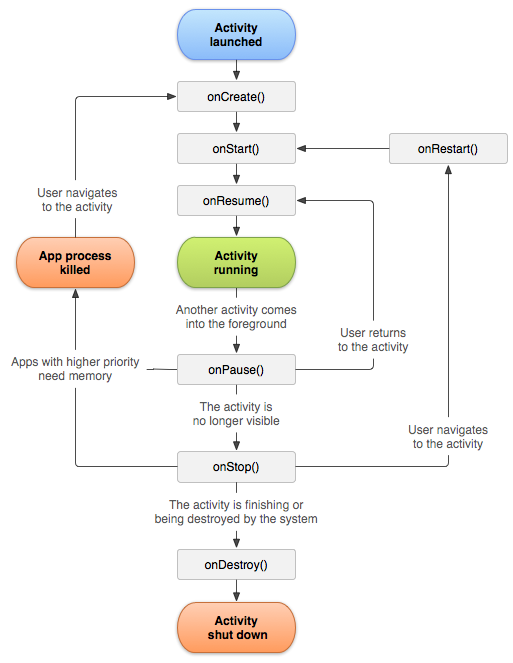
\includegraphics[width=\textwidth,height=0.5\textheight,keepaspectratio]{activity_lifecycle.png}
            \caption{Ciclo de vida de uma \tit{Activity}. Fonte: Android Developer (2021). Disponível em: \url{https://developer.android.com/reference/android/app/Activity}.}
            \label{fig:activy_lifecycle}
        \end{figure}
    
    \paragraph{Service}
    \tit{Services} são componentes muito relevantes quando se trata de realizar tarefas em plano de fundo. Existem três tipos de \tit{Services}:\cite{android:services-overview}
    \begin{itemize}[]
        \item \tit{Foreground:} \tit{Services} em que usuários são notificados que estão em execução. Geralmente acompanham uma notificação na tela. Alguns exemplos de uso comuns são o backup diário do \tit{Whatsapp} ou a sincronização do Gmail para Android. Isto é, são úteis para atividades de segundo plano que necessitam de prioridade e da atenção do usuário.
        \item \tit{Background:} Serviço que roda sem notificação do usuário. Muito embora seja útil para muitos casos, a documentação oficial desencoraja seu uso devido uma série de restrições de processamento em plano de fundo.
        \item \tit{Bound:} Vincula-se este serviço à outro componente através de uma interface de interação inter-processos permitindo assim a interação entre esses, por exemplo, para enviar requisições e receber resultados.
    \end{itemize}
 
    A implementação de um Serviço é muito similar à de uma Atividade. Deve-se estender a classe abstrata \codeword{android.app.Service}. Por ser uma classe abstrata, deve-se sobrescrever necessariamente o método \codeword{onBind(Intent)} que servirá para realizar as interações entre componentes. Para os demais casos, sobrescreve-se os métodos de ciclo de vida do Serviço conforme a necessidade.\cite{android:service}
    
        \begin{lstlisting}[style=Java]
public class MyService extends Service {
    @Override
    public IBinder onBind(Intent intent) {}
    
    @Override
    public void onCreate() {}
    
    @Override
    public int onStartCommand(Intent intent, int flags, int startId) {}
}
    \end{lstlisting}
    
    O ciclo de vida de um \tit{Service} está representado na imagem \ref{fig:service_lifecycle}. O método \codeword{onCreate()} é chamado quando o sistema cria o \tit{Service} e o \codeword{onDestroy()} quando ele o destrói. O \codeword{onStartCommand()} é executado quando um \tit{Service} recebe um comando para começar sua execução \codeword{Context.startService(Intent)}. Este fica executando até parar ou receber um sinal de parada. Por fim, o \codeword{onBind(Intent)} é recebido quando algum outro componente deseja se vincular com este serviço, através do \codeword{Context.bindService(Intent)}.\cite{android:service}
    
       
   \begin{figure}[!ht]
        \centering
        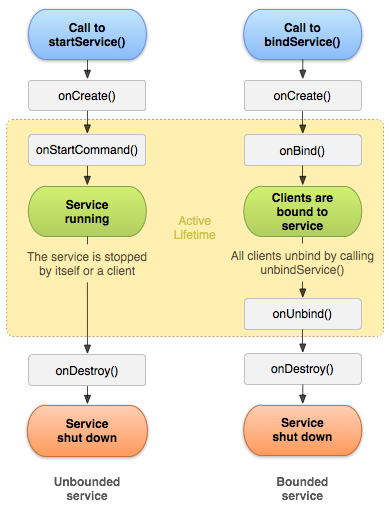
\includegraphics[width=\textwidth,height=0.4\textheight,keepaspectratio]{service_lifecycle.png}
        \caption{Ciclo de vida de um \tit{Service}. Fonte: Android Developer (2021). Disponível em: \url{https://developer.android.com/guide/components/services}.}
        \label{fig:service_lifecycle}
    \end{figure}
    
    \paragraph{BroadcastReceiver}
    O \tit{BroadcastReceiver} é o mais simples de todos os componentes. Ele irá entrar em execução quando algum evento acontecer. Um \tit{BroadcastReceiver} pode ser utilizado para agendar e receber alarmes de sistema ou para eventos do dispositivo como \codeword{BOOT_COMPLETE}.\cite{android:broadcasts-overview}
   
    A implementação do \tit{BroadcastReceiver} envolve a especialização da classe abstrata \\ \codeword{android.content.BroadcastReceiver}. Dessa forma, faz-se necessário a implementação do método \codeword{onReceive(Context, Intent)}.\cite{android:broadcasts-overview}
        
        \begin{lstlisting}[style=Java]
public class MyReceiver extends BroadcastReceiver {
    @Override
    public void onReceive(Context context, Intent intent) {
    }
}
    \end{lstlisting}
    
    
    \subsubsection{Declaração de Componentes de Aplicação}
    A fim de utilizar os componentes de aplicação supra-citados, faz-se necessário declará-los através do \tit{Manifest} da aplicação. No exemplo abaixo, pode-se notar a presença dos 3:
    \begin{lstlisting}[style=Xml]
    <uses-permission android:name="android.permission.RECEIVE_BOOT_COMPLETED" />
    <application
        <activity android:name=".MainActivity"
                  android:exported="true">
            <intent-filter>
                <action android:name="android.intent.action.MAIN"/>
                <category android:name="android.intent.category.LAUNCHER"/>
            </intent-filter>
        </activity>
        
         <service android:name=".MyService" android:enabled="true" 
                android:exported="true" android:process=".myownprocess">
        </service>
        
        <receiver android:enabled="true" android:name=".MyReceiver" android:exported="true">
            <intent-filter>
                <action android:name="android.intent.action.BOOT_COMPLETED"/>
            </intent-filter>
        </receiver>
    </application>
    \end{lstlisting}
    Neste exemplo, temos uma \tit{Activity} que será a tela principal da aplicação e executar-se-á na inicialização da aplicação, temos um \tit{Service} que tem o atributo \codeword{android:process} que irá indicar que ele terá um processo separado do processo padrão da aplicação principal e teremos um \tit{Receiver} que irá ser executado assim que o Sistema Operacional finalizar sua inicialização.
    O atributo \codeword{android:process}, embora tenha sido utilizado no exemplo em uma \tit{Service}, também pode ser utilizado em \tit{Activities} e em \tit{BroadcastReceivers}.\cite{android:activity, android:service, android:broadcasts-overview, android:activity-element, android:service-element, android:receiver-element}
    
    \subsubsection{Comunicação Inter-Processos}
    A comunicação inter-processos pode ser dada através de três mecanismos principais:\cite{stack:ipc}
    \begin{enumerate}
        \item \tit{Intents} são mensagens que um componente pode utilizar para receber e enviar dados e ações, isto é, um mecanismo universal de passagem de dados entre processos. \tit{Intents} utilizam \tit{Bundles} dentro deles para a serialização dos dados passados.\cite{android:intent}
        \item \tit{Bundles} são entidades de dados transmitidos, muito similares à serialização de um objeto.\cite{android:bundle}
        \item \tit{Binders}, já citado, permitem que processos se interliguem através de referências à outros processos.\cite{android:ibinder}
    \end{enumerate}
    
    \subsubsection{Classe Process}
    A Classe \codeword{android.os.Process} do Android SDK dá aos desenvolvedores um conjunto de métodos para os desenvolvedores sobre informações de processos. Dentre as funções que oferece, temos \codeword{Process.myPid()} e \codeword{Process.getElapsedCpuTime()} que, respectivamente, fornece o PID (Identificador de Processo do processo em execução) e o tempo que o processo corrente está em execução.\cite{android:process}
    
    \subsection{Do ponto de vista do Usuário}
    O usuário pode ver, bem como destruí-las com um simples gesto, as atividades que estão em execução através do menu de aplicações recentes, como na figura \ref{fig:recent_apps}. Além disso, ele também pode verificar quais serviços em primeiro-plano estão executando, figura \ref{fig:foreground_services}.
   \begin{figure}[!ht]
        \centering
        \hfill
        \begin{subfigure}{0.3\textwidth}
            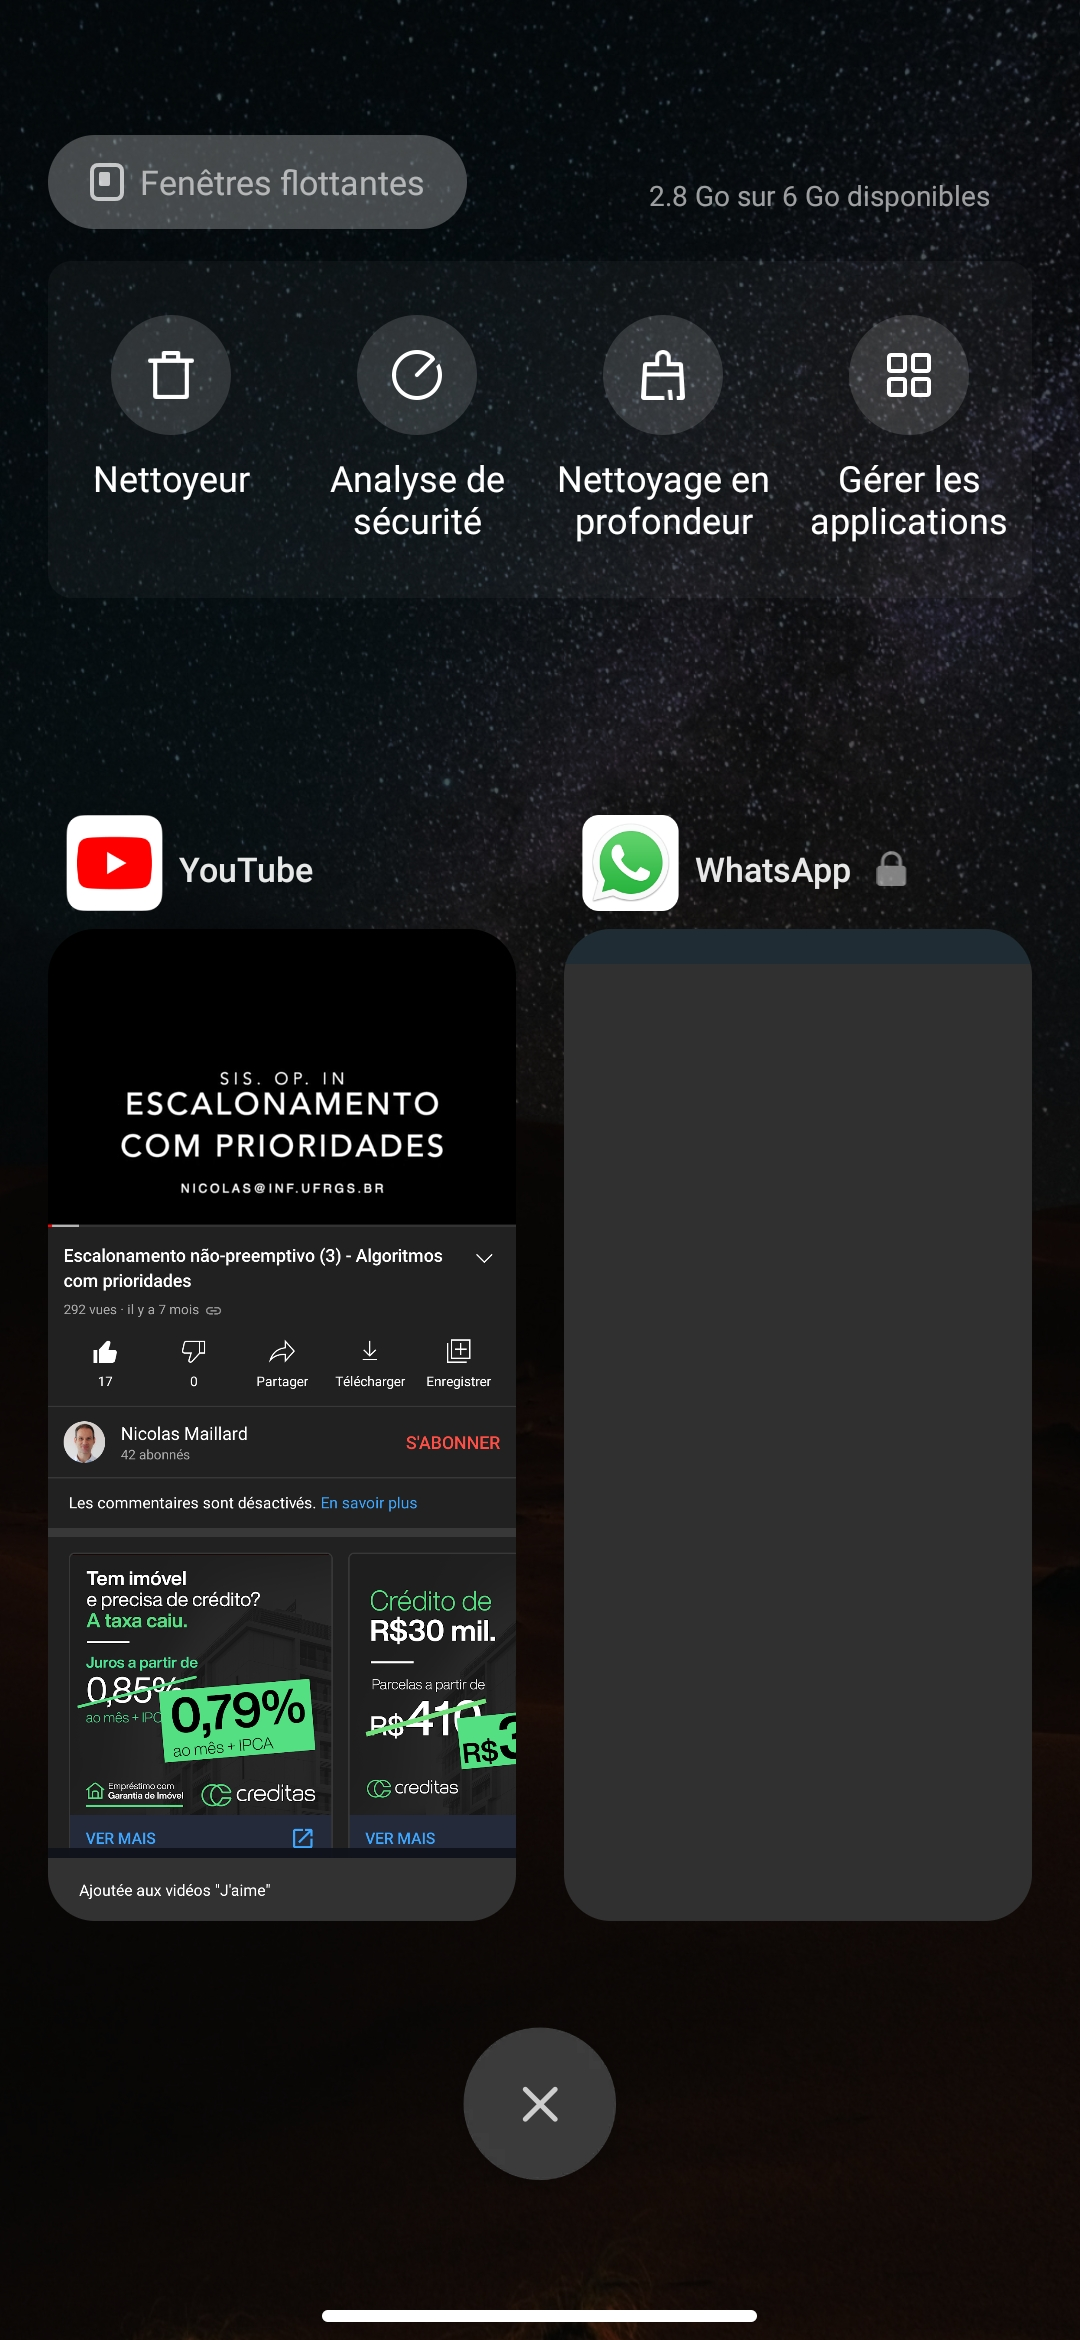
\includegraphics[width=\textwidth,height=0.3\textheight,keepaspectratio]{recents_apps.jpg}
            \caption{Aplicativos em Execução.}
            \label{fig:recent_apps}
        \end{subfigure}
        \hfill
        \begin{subfigure}{0.3\textwidth}
            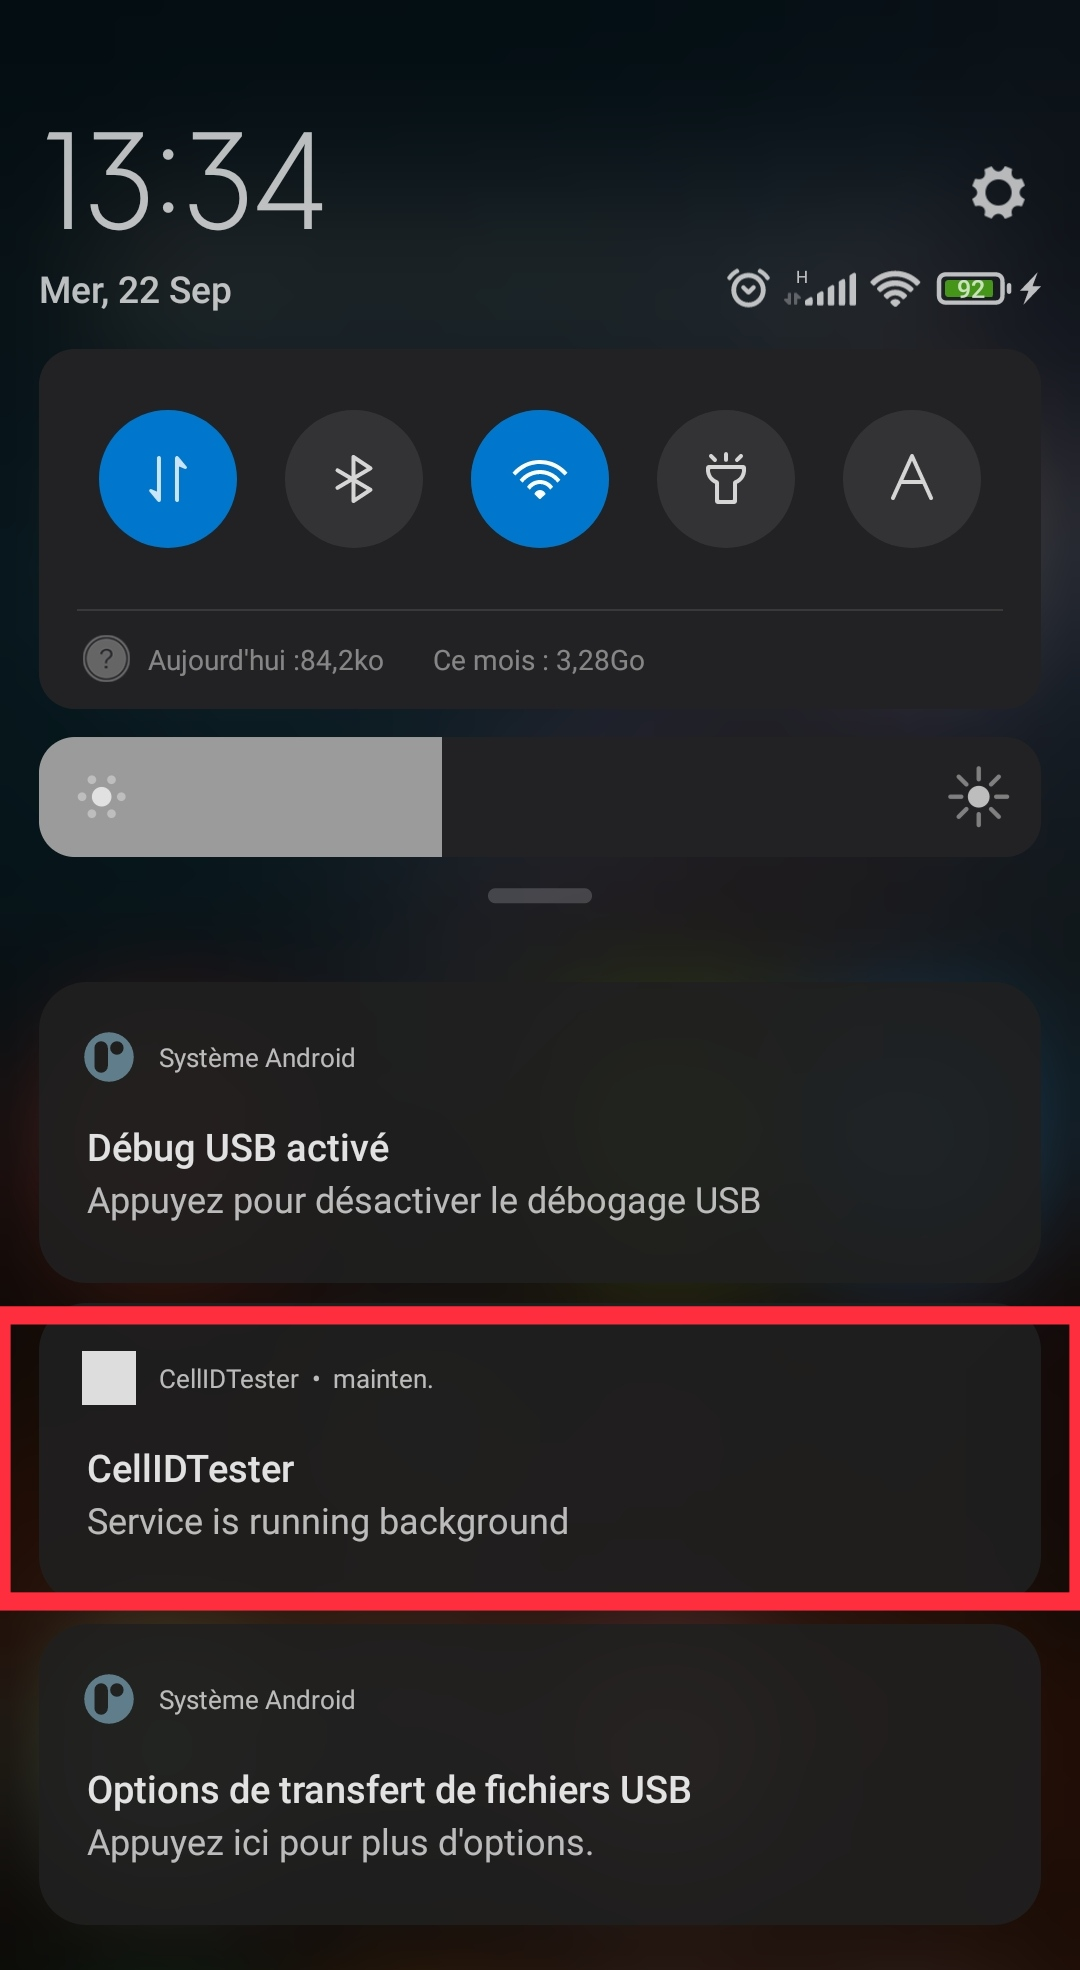
\includegraphics[width=\textwidth,height=0.3\textheight,keepaspectratio]{foreground_service.jpg}
            \caption{Serviço de primeiro plano em execução.}
            \label{fig:foreground_services}
        \end{subfigure}
        \hfill
        \caption{Aplicativos e Serviço de Primeiro-Plano em execução. Fonte: O Autor (2021).}
        \label{fig:user}
    \end{figure}
    
    
    %  Aqui dá pra falar de verificação de processos do sistema
    % Aqui dá pra falar dos Foreground Services
    
    \section{Monitoramento de Processos}
    Enquanto sistema baseado em Linux e, portanto, um sistema Unix, o Android tem diferentes formas de monitorar e visualizar processos através de ferramentas Unix. Em ambientes Unix, a leitura do arquivo virtual \codeword{/proc/stat} e o comando \codeword{top} - e suas variações - são abordagens clássicas para observar as estatísticas de uso de processos. 
    
    Essas abordagens também são possível no Android através do uso de uma ferramenta chamada de \codeword{adb} - \tit{Android Debug Bridge} -, que é muito comum quando se trata de desenvolvimento. O adb disponibiliza diversos recursos para comunicação com o dispositivo tal como executar comandos em um ambiente de shell diretamente no dispositivo através da execução de \codeword{adb shell}.
    
    Muito embora, o \tit{adb} necessite uma permissão específica no dispositivo e seja voltado para desenvolvedores, nele é possível fazer esse \tit{hard use} e utilizar as ferramentas Unix de monitoramento de processos.
    Nas figuras \ref{fig:catprocstat} e \ref{fig:top}, verifica-se, respectivamente, a execução do \codeword{cat /proc/stat} e do comando \codeword{top} no adb shell.
    
    \begin{figure}[!ht]
        \centering
        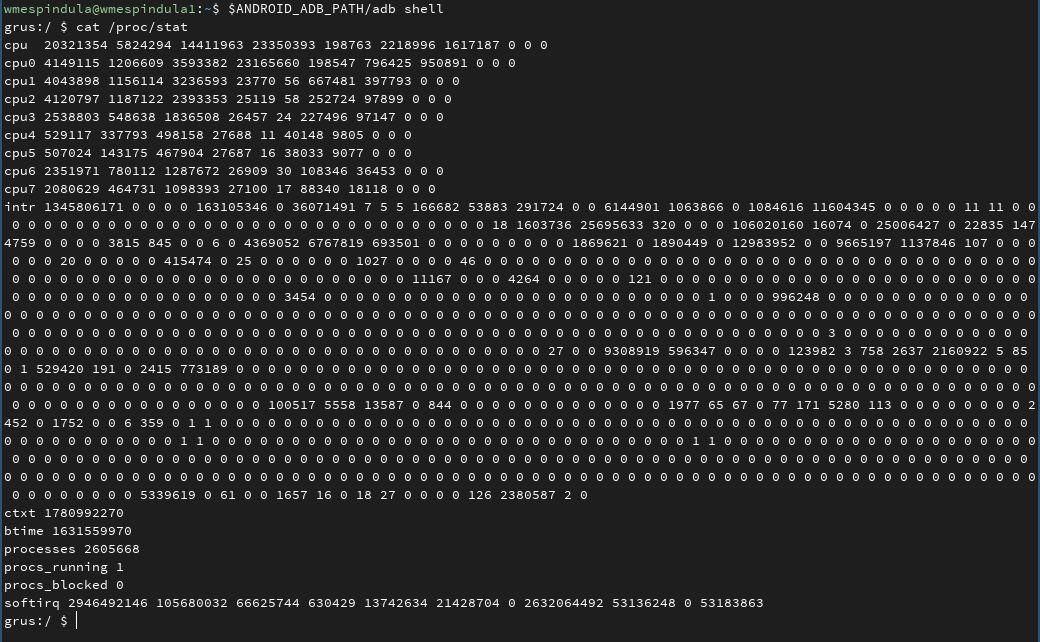
\includegraphics[width=\textwidth,height=0.3\textheight,keepaspectratio]{adb-proc-stat.png}
        \caption{Execução do comando ``cat /proc/stat'' no adb shell. Fonte: O Autor (2021).}
        \label{fig:catprocstat}
    \end{figure}
    
    \begin{figure}[!ht]
        \centering
        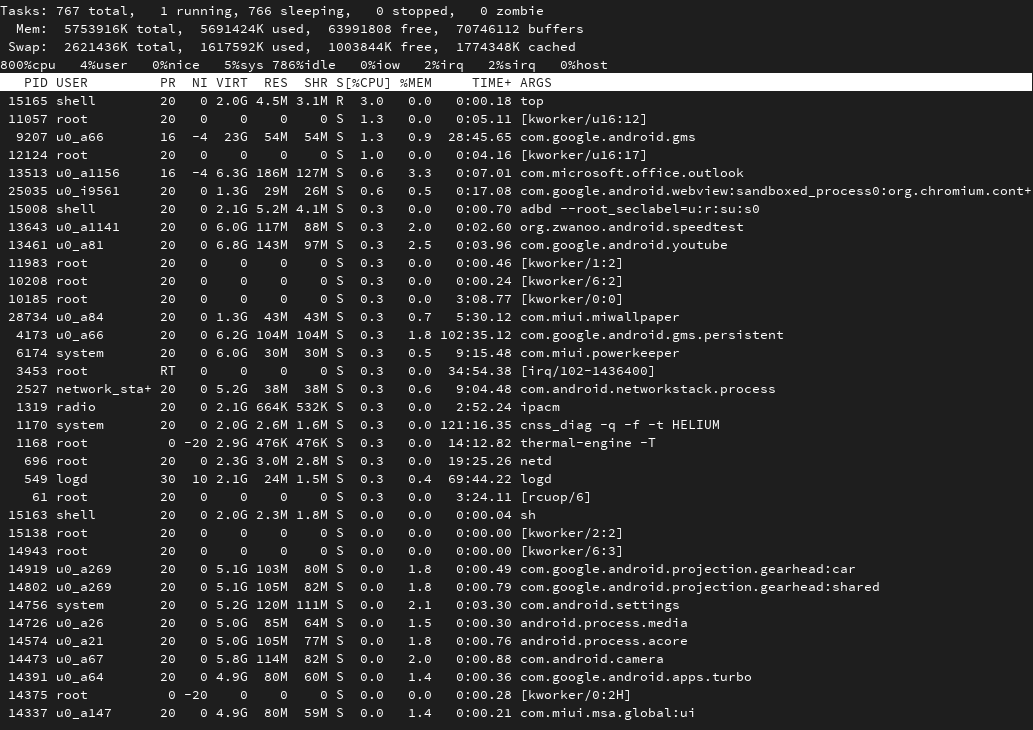
\includegraphics[width=\textwidth,height=0.35\textheight,keepaspectratio]{adb-top.png}
        \caption{Execução do comando ``top'' no adb shell. Fonte: O Autor (2021).}
        \label{fig:top}
    \end{figure}

\clearpage

\nocite{android:processes-and-threads}
\bibliography{ref.bib}

\end{document}